
%% bare_conf.tex
%% V1.3
%% 2007/01/11
%% by Michael Shell
%% See:
%% http://www.michaelshell.org/
%% for current contact information.
%%
%% This is a skeleton file demonstrating the use of IEEEtran.cls
%% (requires IEEEtran.cls version 1.7 or later) with an IEEE conference paper.
%%
%% Support sites:
%% http://www.michaelshell.org/tex/ieeetran/
%% http://www.ctan.org/tex-archive/macros/latex/contrib/IEEEtran/
%% and
%% http://www.ieee.org/

%%*************************************************************************
%% Legal Notice:
%% This code is offered as-is without any warranty either expressed or
%% implied; without even the implied warranty of MERCHANTABILITY or
%% FITNESS FOR A PARTICULAR PURPOSE! 
%% User assumes all risk.
%% In no event shall IEEE or any contributor to this code be liable for
%% any damages or losses, including, but not limited to, incidental,
%% consequential, or any other damages, resulting from the use or misuse
%% of any information contained here.
%%
%% All comments are the opinions of their respective authors and are not
%% necessarily endorsed by the IEEE.
%%
%% This work is distributed under the LaTeX Project Public License (LPPL)
%% ( http://www.latex-project.org/ ) version 1.3, and may be freely used,
%% distributed and modified. A copy of the LPPL, version 1.3, is included
%% in the base LaTeX documentation of all distributions of LaTeX released
%% 2003/12/01 or later.
%% Retain all contribution notices and credits.
%% ** Modified files should be clearly indicated as such, including  **
%% ** renaming them and changing author support contact information. **
%%
%% File list of work: IEEEtran.cls, IEEEtran_HOWTO.pdf, bare_adv.tex,
%%                    bare_conf.tex, bare_jrnl.tex, bare_jrnl_compsoc.tex
%%*************************************************************************

% *** Authors should verify (and, if needed, correct) their LaTeX system  ***
% *** with the testflow diagnostic prior to trusting their LaTeX platform ***
% *** with production work. IEEE's font choices can trigger bugs that do  ***
% *** not appear when using other class files.                            ***
% The testflow support page is at:
% http://www.michaelshell.org/tex/testflow/



% Note that the a4paper option is mainly intended so that authors in
% countries using A4 can easily print to A4 and see how their papers will
% look in print - the typesetting of the document will not typically be
% affected with changes in paper size (but the bottom and side margins will).
% Use the testflow package mentioned above to verify correct handling of
% both paper sizes by the user's LaTeX system.
%
% Also note that the "draftcls" or "draftclsnofoot", not "draft", option
% should be used if it is desired that the figures are to be displayed in
% draft mode.
%
\documentclass[conference,compsoc,letterpaper]{IEEEtran}
% Add the compsoc option for Computer Society conferences.
%
% If IEEEtran.cls has not been installed into the LaTeX system files,
% manually specify the path to it like:
% \documentclass[conference]{../sty/IEEEtran}

\newcommand{\CLASSINPUTinnersidemargin}{1in} 
\newcommand{\CLASSINPUToutersidemargin}{1in} 


% Some very useful LaTeX packages include:
% (uncomment the ones you want to load)


% *** MISC UTILITY PACKAGES ***
%
\usepackage{ifpdf}
% Heiko Oberdiek's ifpdf.sty is very useful if you need conditional
% compilation based on whether the output is pdf or dvi.
% usage:
% \ifpdf
%   % pdf code
% \else
%   % dvi code
% \fi
% The latest version of ifpdf.sty can be obtained from:
% http://www.ctan.org/tex-archive/macros/latex/contrib/oberdiek/
% Also, note that IEEEtran.cls V1.7 and later provides a builtin
% \ifCLASSINFOpdf conditional that works the same way.
% When switching from latex to pdflatex and vice-versa, the compiler may
% have to be run twice to clear warning/error messages.




% *** CITATION PACKAGES ***
%
%\usepackage{cite}
% cite.sty was written by Donald Arseneau
% V1.6 and later of IEEEtran pre-defines the format of the cite.sty package
% \cite{} output to follow that of IEEE. Loading the cite package will
% result in citation numbers being automatically sorted and properly
% "compressed/ranged". e.g., [1], [9], [2], [7], [5], [6] without using
% cite.sty will become [1], [2], [5]--[7], [9] using cite.sty. cite.sty's
% \cite will automatically add leading space, if needed. Use cite.sty's
% noadjust option (cite.sty V3.8 and later) if you want to turn this off.
% cite.sty is already installed on most LaTeX systems. Be sure and use
% version 4.0 (2003-05-27) and later if using hyperref.sty. cite.sty does
% not currently provide for hyperlinked citations.
% The latest version can be obtained at:
% http://www.ctan.org/tex-archive/macros/latex/contrib/cite/
% The documentation is contained in the cite.sty file itself.




% *** GRAPHICS RELATED PACKAGES ***
%
\ifpdf
  \usepackage[pdftex]{graphicx}
  % declare the path(s) where your graphic files are
  \graphicspath{{../pdf/}{../jpeg/}{img/}}
  % and their extensions so you won't have to specify these with
  % every instance of \includegraphics
  \DeclareGraphicsExtensions{.pdf,.jpeg,.png}
\else
  % or other class option (dvipsone, dvipdf, if not using dvips). graphicx
  % will default to the driver specified in the system graphics.cfg if no
  % driver is specified.
  \usepackage[dvips]{graphicx}
  % declare the path(s) where your graphic files are
  \graphicspath{{../eps/}}
  % and their extensions so you won't have to specify these with
  % every instance of \includegraphics
  \DeclareGraphicsExtensions{.eps}
\fi% graphicx was written by David Carlisle and Sebastian Rahtz. It is
% required if you want graphics, photos, etc. graphicx.sty is already
% installed on most LaTeX systems. The latest version and documentation can
% be obtained at: 
% http://www.ctan.org/tex-archive/macros/latex/required/graphics/
% Another good source of documentation is "Using Imported Graphics in
% LaTeX2e" by Keith Reckdahl which can be found as epslatex.ps or
% epslatex.pdf at: http://www.ctan.org/tex-archive/info/
%
% latex, and pdflatex in dvi mode, support graphics in encapsulated
% postscript (.eps) format. pdflatex in pdf mode supports graphics
% in .pdf, .jpeg, .png and .mps (metapost) formats. Users should ensure
% that all non-photo figures use a vector format (.eps, .pdf, .mps) and
% not a bitmapped formats (.jpeg, .png). IEEE frowns on bitmapped formats
% which can result in "jaggedy"/blurry rendering of lines and letters as
% well as large increases in file sizes.
%
% You can find documentation about the pdfTeX application at:
% http://www.tug.org/applications/pdftex





% *** MATH PACKAGES ***
%
\usepackage[cmex10]{amsmath}
% A popular package from the American Mathematical Society that provides
% many useful and powerful commands for dealing with mathematics. If using
% it, be sure to load this package with the cmex10 option to ensure that
% only type 1 fonts will utilized at all point sizes. Without this option,
% it is possible that some math symbols, particularly those within
% footnotes, will be rendered in bitmap form which will result in a
% document that can not be IEEE Xplore compliant!
%
% Also, note that the amsmath package sets \interdisplaylinepenalty to 10000
% thus preventing page breaks from occurring within multiline equations. Use:
\interdisplaylinepenalty=2500
% after loading amsmath to restore such page breaks as IEEEtran.cls normally
% does. amsmath.sty is already installed on most LaTeX systems. The latest
% version and documentation can be obtained at:
% http://www.ctan.org/tex-archive/macros/latex/required/amslatex/math/

% ADDED BY BOLSTER
\usepackage{amssymb}




% *** SPECIALIZED LIST PACKAGES ***
%
%\usepackage{algorithmic}
% algorithmic.sty was written by Peter Williams and Rogerio Brito.
% This package provides an algorithmic environment fo describing algorithms.
% You can use the algorithmic environment in-text or within a figure
% environment to provide for a floating algorithm. Do NOT use the algorithm
% floating environment provided by algorithm.sty (by the same authors) or
% algorithm2e.sty (by Christophe Fiorio) as IEEE does not use dedicated
% algorithm float types and packages that provide these will not provide
% correct IEEE style captions. The latest version and documentation of
% algorithmic.sty can be obtained at:
% http://www.ctan.org/tex-archive/macros/latex/contrib/algorithms/
% There is also a support site at:
% http://algorithms.berlios.de/index.html
% Also of interest may be the (relatively newer and more customizable)
% algorithmicx.sty package by Szasz Janos:
% http://www.ctan.org/tex-archive/macros/latex/contrib/algorithmicx/
\usepackage{algpseudocode}




% *** ALIGNMENT PACKAGES ***
%
%\usepackage{array}
% Frank Mittelbach's and David Carlisle's array.sty patches and improves
% the standard LaTeX2e array and tabular environments to provide better
% appearance and additional user controls. As the default LaTeX2e table
% generation code is lacking to the point of almost being broken with
% respect to the quality of the end results, all users are strongly
% advised to use an enhanced (at the very least that provided by array.sty)
% set of table tools. array.sty is already installed on most systems. The
% latest version and documentation can be obtained at:
% http://www.ctan.org/tex-archive/macros/latex/required/tools/


\usepackage{mdwmath}
\usepackage{mdwtab}
% Also highly recommended is Mark Wooding's extremely powerful MDW tools,
% especially mdwmath.sty and mdwtab.sty which are used to format equations
% and tables, respectively. The MDWtools set is already installed on most
% LaTeX systems. The lastest version and documentation is available at:
% http://www.ctan.org/tex-archive/macros/latex/contrib/mdwtools/


% IEEEtran contains the IEEEeqnarray family of commands that can be used to
% generate multiline equations as well as matrices, tables, etc., of high
% quality.


%\usepackage{eqparbox}
% Also of notable interest is Scott Pakin's eqparbox package for creating
% (automatically sized) equal width boxes - aka "natural width parboxes".
% Available at:
% http://www.ctan.org/tex-archive/macros/latex/contrib/eqparbox/





% *** SUBFIGURE PACKAGES ***
%\usepackage[tight,footnotesize]{subfigure}
% subfigure.sty was written by Steven Douglas Cochran. This package makes it
% easy to put subfigures in your figures. e.g., "Figure 1a and 1b". For IEEE
% work, it is a good idea to load it with the tight package option to reduce
% the amount of white space around the subfigures. subfigure.sty is already
% installed on most LaTeX systems. The latest version and documentation can
% be obtained at:
% http://www.ctan.org/tex-archive/obsolete/macros/latex/contrib/subfigure/
% subfigure.sty has been superceeded by subfig.sty.



%\usepackage[caption=false]{caption}
%\usepackage[font=footnotesize]{subfig}
% subfig.sty, also written by Steven Douglas Cochran, is the modern
% replacement for subfigure.sty. However, subfig.sty requires and
% automatically loads Axel Sommerfeldt's caption.sty which will override
% IEEEtran.cls handling of captions and this will result in nonIEEE style
% figure/table captions. To prevent this problem, be sure and preload
% caption.sty with its "caption=false" package option. This is will preserve
% IEEEtran.cls handing of captions. Version 1.3 (2005/06/28) and later 
% (recommended due to many improvements over 1.2) of subfig.sty supports
% the caption=false option directly:
\usepackage[caption=false,font=footnotesize]{subfig}
%
% The latest version and documentation can be obtained at:
% http://www.ctan.org/tex-archive/macros/latex/contrib/subfig/
% The latest version and documentation of caption.sty can be obtained at:
% http://www.ctan.org/tex-archive/macros/latex/contrib/caption/




% *** FLOAT PACKAGES ***
%
%\usepackage{fixltx2e}
% fixltx2e, the successor to the earlier fix2col.sty, was written by
% Frank Mittelbach and David Carlisle. This package corrects a few problems
% in the LaTeX2e kernel, the most notable of which is that in current
% LaTeX2e releases, the ordering of single and double column floats is not
% guaranteed to be preserved. Thus, an unpatched LaTeX2e can allow a
% single column figure to be placed prior to an earlier double column
% figure. The latest version and documentation can be found at:
% http://www.ctan.org/tex-archive/macros/latex/base/



%\usepackage{stfloats}
% stfloats.sty was written by Sigitas Tolusis. This package gives LaTeX2e
% the ability to do double column floats at the bottom of the page as well
% as the top. (e.g., "\begin{figure*}[!b]" is not normally possible in
% LaTeX2e). It also provides a command:
%\fnbelowfloat
% to enable the placement of footnotes below bottom floats (the standard
% LaTeX2e kernel puts them above bottom floats). This is an invasive package
% which rewrites many portions of the LaTeX2e float routines. It may not work
% with other packages that modify the LaTeX2e float routines. The latest
% version and documentation can be obtained at:
% http://www.ctan.org/tex-archive/macros/latex/contrib/sttools/
% Documentation is contained in the stfloats.sty comments as well as in the
% presfull.pdf file. Do not use the stfloats baselinefloat ability as IEEE
% does not allow \baselineskip to stretch. Authors submitting work to the
% IEEE should note that IEEE rarely uses double column equations and
% that authors should try to avoid such use. Do not be tempted to use the
% cuted.sty or midfloat.sty packages (also by Sigitas Tolusis) as IEEE does
% not format its papers in such ways.





% *** PDF, URL AND HYPERLINK PACKAGES ***
%
%\usepackage{url}
% url.sty was written by Donald Arseneau. It provides better support for
% handling and breaking URLs. url.sty is already installed on most LaTeX
% systems. The latest version can be obtained at:
% http://www.ctan.org/tex-archive/macros/latex/contrib/misc/
% Read the url.sty source comments for usage information. Basically,
% \url{my_url_here}.





% *** Do not adjust lengths that control margins, column widths, etc. ***
% *** Do not use packages that alter fonts (such as pslatex).         ***
% There should be no need to do such things with IEEEtran.cls V1.6 and later.
% (Unless specifically asked to do so by the journal or conference you plan
% to submit to, of course. )


% correct bad hyphenation here
\hyphenation{op-tical net-works semi-conduc-tor}

%%%%%%%%%%%%%%%%%%%%%%%%%%%%%%%%%%%
% BOLSTER PACKAGES FOR DEV PERIOD %
%%%%%%%%%%%%%%%%%%%%%%%%%%%%%%%%%%%
\usepackage{booktabs}
\usepackage{tabularx}
%\usepackage{hyperref}
\usepackage{todonotes}
\presetkeys%
    {todonotes}%
    {inline,backgroundcolor=yellow}{}

\graphicspath{{../../../Figures/}{./figures/}}

%\usepackage{fancyhdr}
%\fancypagestyle{firstpage}{% Page style for first page
%  \fancyhf{}% Clear header/footer
%  \renewcommand{\headrulewidth}{0.4pt}% Header rule
%  \fancyhead[C]{Draft for Submission to Mobile Adhoc Sensor Systems (MASS'16) Brasilia Oct'16}% Header
%}
%\pagestyle{plain}% Default page style


\begin{document}

%
% paper title
% can use linebreaks \\ within to get better formatting as desired
\title{Physical Behaviours for Trust Assessment in Autonomous Underwater MANETs}


% author names and affiliations
% use a multiple column layout for up to three different
% affiliations
\author{\IEEEauthorblockN{Andrew Bolster}
\IEEEauthorblockA{Department of Electrical Engineering and Electronics\\
University of Liverpool\\
Liverpool, UK\\
Email: bolster@liv.ac.uk}
\and
\IEEEauthorblockN{Alan Marshall}
\IEEEauthorblockA{Department of Electrical Engineering and Electronics\\
University of Liverpool\\
Liverpool, UK\\
Email: alan.marshall@liv.ac.uk}
}

% use for special paper notices
%\IEEEspecialpapernotice{Pages: 9, Deadline: 25/3}




% make the title area
\maketitle

%\thispagestyle{firstpage}% firstpage page style for first page


\begin{abstract}
%\boldmath

%\emph{Relevant sections from the \href{http://www.ene.unb.br/mass2016/}{CFP} art: Key Mgmt \& Trust Establishment; Robotic Networks; Vehicular Networks \& Protocols; Location Based Services; Mobility Managment}

This paper proposes a new approach to trust in resource-constrained networks of autonomous systems based on their physical behaviour, using the motion of nodes within a team to detect and potentially identify malicious or failing operation within a cohort.
This is accomplished by looking specifically at operations within the three dimensions of the underwater space.
We present a series of composite metrics based on physical movement, and apply these metrics to the detection and discrimination of sample physical misbehaviours.
This approach opens the possibility of bringing information about both the physical and communications behaviours of autonomous MANETs together to strengthen and expand the application of future Trust Management Frameworks in sparse and/or resource constrained environments.

\end{abstract}
% no keywords

% For peer review papers, you can put extra information on the cover
% page as needed:
% \ifCLASSOPTIONpeerreview
% \begin{center} \bfseries EDICS Category: 3-BBND \end{center}
% \fi
%
% For peerreview papers, this IEEEtran command inserts a page break and
% creates the second title. It will be ignored for other modes.
\IEEEpeerreviewmaketitle



\section{Introduction}

Early attempts to secure and protect the integrity of Mobile Ad-hoc Networks have relied on various forms of strong-cryptography to protect information being transferred from tampering or malicious inspection.
While such approaches protect the integrity of individual pieces of data, the increased computation, and storage requirements of modern, strong, decentralised cryptographic systems presents a clear avenue for Denial of Service (DoS) attacks on MANETs.
This threat is particularly relevant in resource-constrained networks, where one or more aspects of the environment are limited, be it available power, mobility, data storage, onboard processing, bandwidth, and channel resources such as capacity and delay.
In such networks, where there is a requirement of security and/or integrity monitoring, strong-cryptographic methods present an entirely new opportunity to potential attackers.

One solution to the trade-off between DoS-protection, and security is the assessment of ``trustworthiness'' of nodes within a local network. 
``Trust'' in this case is an assessment of capability of a node based on previously observed behaviour.
Using this Trust to make simple routing decisions is significantly simpler and faster that strong-cryptographic methods, particularly in multi-hop networks or resource constrained networks\cite{Cordasco2008}.
With Trust being reliant on the near-real-time awareness of some behaviour, and cryptography on the pre-establishment of some entropy store and the repeated reinforcement of that numerical security, they represent two very different approaches to system integrity with very different costs/benefits and in practice, some elements of both methodologies will be used in different contexts and applications. 

However, these approaches to operational security have been totally focused on the establishment of trust/security in the communications domain, and ignore other potential threats to the network exploited through physical movement.
This threat is particularly evident in collaborative autonomous systems where nodes are tasked to accomplish some survey / exploration / observation objective in a distributed fashion, where individual nodes make decisions based on the actions of their ``team''. 
This collaboration opens the opportunity for a physically-misbehaving actor to selfishly conserve it's own resources, or maliciously ``drain'' a given target node.
Current security / trust systems applied to MANETs are not concerned with the threat of such physical misbehaviours.

This paper proposes a new approach to trust in resource-constrained networks of autonomous systems based on their physical behaviour, assessing the viability of using the motion of nodes within a team to detect and potentially identify malicious or failing operation within a cohort.
This is accomplished by looking specifically at operations within the three dimensions of the underwater space.

In the majority of Trusted autonomous mobile network implementations, a free space RF communications protocol such as 802.11 is used as the source of all information about the trustworthy operation of the network.
Most such trust frameworks use a single type of observed communication action to derive trust assessments, typically successfully delivered or forwarded packets. 
By their nature, such implementations rely on relatively high bandwidth, low noise, low latency, and high channel occupancy where contention is tolerable.
In contrast; in underwater environments, communications is sparse, delayful, noisy, and very prone to destructive contention.
Therefore, observations of the communications processes used to assess trust occur much less frequently, with much greater error (noise) and delay than is experienced in terrestrial RF MANETS.
In addition to the communications challenges, other considerations such as command and control isolation, as well as power and locomotive limitations, and the increasing drive towards the use of teams of smaller, cheaper, almost disposable autonomous underwater vehicles (AUVs), particularly in defence, ecological and petrochemical fields, present unique threats against trust management. 

In Section~\ref{sec:mobility}, we review the current use cases, deployments and mobility patterns of collaborative AUV operations, and the state-of-the-art in underwater localisation techniques.
In Section~\ref{sec:tmfs}, we discuss the use of Trust Management Frameworks and their relevance and applicability to marine operations. 
In Section~\ref{sec:physbev}, we propose a collection of metrics to characterise the physical behaviours of node, and establish a set of physical ``misbehaviours'' to test these against.
In Section~\ref{sec:sim_and_valid}, we design a series of simulations, and tests to assess the detection and identification capabilities of three potential physical metrics for trust assessment.


\section{AUV Mobility and Localisation}\label{sec:mobility}

The use and applications of Autonomous Underwater Vehicles (AUVs) has undergone a great expansion in recent years; current applications and considerations are summarised below.


\subsection{AUV operations and deployments}

\subsubsection{Hydrographic Survey}

The use of AUVs in the place of manned-surface platforms or tethered undersea platforms enables greatly increased spatial and temporal sampling.
Importantly, the separation of AUVs from the noisy sea surface enables much more efficient survey operations.
This is particularly important when comparing to classical tow-line based measurements; where the mobility of the AUVs enables for much tighter-turning survey patterns or operation in inaccessible or hard-to-reach locations such as polar survey\cite{Curtin1993}.

Another significant factor is cost; the daily cost of operating a manned vessel can be considerably higher than the costs of deploying, operating and recovering one or more AUVs with equivalent capabilities\cite{Nicholson2008}.
Additionally, the use of low-power ``glider'' AUVs has lowered the barrier to entry for extended mission types, such as persistent environmental survey, or open-ocean operations. 
Depth-hardened AUVs have also opened up the deepest parts of the oceans to exploration, with the onboard autonomy, imagery and Simultaneous Location and Mapping (SLAM) techniques allowing deep-dwelling survey AUVs to react to bottom-surface features without the need for a tight craft-to-surface control loop.
The natural extension of these kind of applications is the use of AUVs on ice-covered planets such as Europa, where three-dimensional, autonomous navigation without an on-the-loop controller is vital for mission resource efficiency and success.

\subsubsection{Hull and Infrastructure Inspection}
Ongoing concerns regarding the security, safety and legality of international shipping has driven the application of AUVs to the area of near-surface hull and infrastructure inspections, looking for damage as well as devices such as limpet mines and other contraband.
This use case puts a range of unique pressures on the AUV system; requiring highly accurate three-dimensional localisation and path-planning to clearly image the contours of a hull\cite{Nicholson2008}.
Similarly, with the increasing use and criticality of intercontinental undersea optical fibre connections, using AUVs for both the laying of and inspection of these cables is an exciting area of work\cite{Yu2004}\cite{Asakawa2002}.

\subsubsection{Marine Petrochemical}
Oil and Gas industry requirements for high quality, low altitude bathymetry of seabed structures for infrastructure development (pipelines/drill platforms etc.) as well as monitoring of those structures over time (inspection etc.) is another significant application area, and a major driver of research investment.
As in Hydrography, the mobility of AUVs is the biggest single advantage over classical platforms\cite{Morr2003}.

\subsubsection{Military}
Mine-Countermeasure Operations benefit greatly from, and significantly drive, AUV development; the ability to rapidly explore and covertly survey a potentially dangerous area without risking a human operator is a major benefit.
This benefit applies to protection as well as incursion; the ability to have persistent survey of a valuable area such as a forward-operating harbour is increasingly essential, and as AUV technology, autonomy and security practices develop, this use is increasing.
This Port Protection capability is particularly complex;  teams of AUVs are expected to repeatedly survey an area and remain densely-connected enough to maintain end-to-end communications with all other nodes, in the face of an environment that is possibly not well surveyed initially, and includes dynamically moving obstacles (i.e.\ ships).
In Sec.~\ref{sec:sim_and_valid}, we use this Port Protection scenario as a baseline for our simplified simulation context.

%\todo{\emph{For Chapter} Look at redoing this with other mobilities (particularly distributed lawnmower)}

\subsection{Localisation Technologies}

Given the subsurface nature of most AUV operations, terrestrial localisation techniques such as GPS are unavailable (below $\approx 20cm$ depth). 
However, a range of alternative techniques are used to maintain spacial awareness to a high degree of accuracy in the underwater environment.
\subsubsection{Long baseline (LBL)}
Long-baseline localisation systems use a series of static surface/cable networked acoustic transponders to provide coordinated beacons and (usually) GPS-backed relative location information to local subsurface users. 
Such systems can be accurate to less that $0.1m$ or better in ideal deployments and are regularly used in controlled autonomous survey environments such as harbour patrol operations where the deployment area is bounded. 
However, the initial setup and deployment required in advance of any AUV operation makes LBL difficult to utilise in unbounded or contended areas.
LBL systems can also be deployed on mobile surface platforms in the area (ships or buoys for example), but these applications put significant computational pressure on the end-point AUV and have greatly reduced accuracy compared to ideal deployments\cite{Matos1999}.
\subsubsection{Doppler Velocity Log (DVL)}
Doppler Velocity Logging involves the emission of directed acoustic ``pings'' that reflect off sea bed/surface interfaces that, when received back on the craft with multi-beam phased array acoustic transducers can measure both the absolute depth/altitude (z-axis) of the craft and through directional Doppler shifting, the relative (xy-translative) motion of the craft since the ping.
While classical DVL was highly sensitive to shifting currents in the water column, advances in the development of Acoustic Doppler Current Profiling has turned that situation on it's head, enabling the compensation-for and measurement-of water currents down to the sub-meter level\cite{Snyder2010}.
\subsubsection{Inertial Navigation Systems (INS)}
Inertial navigation systems use gyroscopic procession to observe the relative acceleration of a mobile platform.
This reference-relative monitoring is particularly useful in the underwater environment, as it detects the motion of AUVs as they are carried by the water itself.
Bias Drift is a significant problem for INS systems operating over longer (hundreds of metres) distances, as they usually have some minimal amount of directional bias, that incurs a cumulative effect over time without assistance.
Several sensor synthesis processes have been demonstrated which combine information from INS along with DVL data to improve localisation into the sub-decimeter level\cite{Jalving2003}\cite{Liu2014}.
\subsubsection{Simultaneous Location and Mapping (SLAM)}
Simultaneous Location and Mapping is the process of iteratively developing a feature-based model of an environment, and to use the relative movement within that modeled environment to obtain estimates of absolute positioning.
SLAM has been most well developed in the contexts of either visual-based inspection using cameras, or LIDAR-style distance triangulation, however the same principles have been successfully applied using marine sonar readings, providing sub-meter accuracy, real-time, feature-relative localisation information that is (for the most part) environmentally agnostic\cite{Williams2000}.

In summary, current technology reliably enables AUVs to localise to a sub-metre accuracy in most areas of application.

\section{Trust Management Frameworks}\label{sec:tmfs}

Trust Management Frameworks (TMFs) provide information to assist the estimation of future states and actions of nodes operating as teams, groups or networks. 
This information is used to optimize the performance of a team against malicious, selfish, or defective misbehaviour by one or more nodes.
Previous research has established the advantages of implementing communications-based TMFs in terrestrial, 802.11 based MANETs, particularly in terms of preventing selfish operation in collaborative systems \cite{Li2007}, and maintaining throughput in the presence of malicious actors \cite{Buchegger2002}. 
These observations then inform future decisions of individual nodes, for example, route selection \cite{Li2008}.

Recent work has demonstrated the use of a number of metrics to form a ``vector'' of trust. The Multi-parameter Trust Framework for MANETs (MTFM) \cite{Guo2012}, uses a range of communications metrics beyond packet delivery/loss rate (PLR) to assess trust. This vectorized trust also allows a system to detect and identify the tactics being used to undermine or subvert trust. 
This method as been previously applied to the marine space, comparing against a selection of existing communications TMFs \cite{Bolster2015} showing that MTFM is more effective at detecting misbehaviours in sparse communications environments. 

\section{Physical Behaviours for Trust}\label{sec:physbev}

\subsection{Physical Metrics}

Three physical metrics are used to encompass the relative distributions and activities of nodes within the network; Inter-node Distance Deviation (INDD), Inter-node Heading Deviation (INHD), and Node Speed. 
Conceptually, INDD is a measure of the average spacing of an observed node with respect to its neighbours. 
INHD is a similar approach with respect to node orientation.
As such, these metrics completely encapsulate and abstract the physical behaviour of any node, potentially performing any misbehaviour.
Given that local nodes within the team are aware of the reported positions and velocities of their neighbours, it is believed that this is a reasonable initial set of metrics to establish the usefulness of physical metrics of trust assessment.

Additional metric constructions may be more suitable for certain contexts, platforms or operations, however these were selected in collaboration with UK DSTL and NATO CMRE as suitable, generic, assessments, viable on most current platforms in most current deployment schemes.


\begin{align}
  INDD_{i,j} &= \frac{|P_j - \sum_x \frac{P_x}{N}|}{\frac{1}{N}\sum_x \sum_y{|P_x - P_y| (\forall x \neq y)}}\\
  INHD_{i,j} &= \hat{v} \vert v= V_j - \sum_x{\frac{V_x}{N}}\\
  V_{i,j} &= |V_j|
\end{align}

Where $i$ and $j$ are indices denoting the current observer node and the current observed node respectively; $x$ is a summation index representing other nodes in the observers region of concern; $P{j}$ is the $[x,y,z]$ absolute position of the observed node (relative to some coordinated origin point agreed upon at launch) and $V{j}$ is the $[x,y,z]$ velocity of the observed node.

Thus, the metric vector used for the physical-trust assessment from one observer node to a given target node is;

\begin{equation}
  X_{i,j}=\{\text{INDD}_{i,j}, \text{INHD}_{i,j},, V_{i,j}\}
  \label{eq:phys_vector}
\end{equation}
At each time-step, each node will have a separate $X$ assessment vector for each node it has observed in that time. 
Ergo the fleet or team as a whole will have $N\times N$ assessment vectors at each timestep.

\subsection{Physical Misbehaviours}
Misbehaviours in the communications space is heavily investigated area in MANETs \cite{Konate2011}\cite{Wang2009}\cite{Chen2014a}\cite{Mitchell2014}, but attacks and misbehaviours in the physical space are far less explored. 
Both in terrestrial and underwater contexts, as MANET applications expand and become increasingly \emph{de rigueur}, the impacts of physical or operational misbehaviour become increasingly relevant. 
As in the communications space, the primary drivers of any ``misbehaviour'' come under two general categories; selfish operation or malicious subterfuge.
Autonomous MANETs in general rely (or are at least, most effective) when all nodes operate fairly, be that in terms of their bandwidth sharing, energy usage, routing optimality or other factors. 
Physically, if a node is being ``selfish'', it may preferentially move to the edge of a network to minimise it's dynamic work allocation, or depending on it's intent, may insert itself into the centre of a network to maximise it's ability to capture, monitor, and manipulate traffic going across the network. 
In the context of a secure operation (or one that's assumed to be secure), the opportunity for capturing a legitimate node and replacing it with a modified clone.
Assuming a highly capable outside actor and a multi-channel communications opportunity, there is also the possibility of a node appearing to ``play along'' with the crowd that occasionally breaks rank to route internal transmissions to a outside agent.
In the underwater context this may mean an AUV following the rest of a team along a survey path and occasionally ``breaking surface'' to communicate to a malicious controller.
Alternatively, if an inserted node is not totally aware of a given mission parameter, such as a particular survey or waypointing path, it may simply follow along, hoping not to be noticed.

In all these cases, such behaviour involves some element of behaving differently from the rest of the team, however, there are other cases where such individual ``deviance'' is observed; where a node is in some kind of mechanical ``failure state''.
In the underwater context, this could be damage to the drive-train or navigation systems, causing it to lag behind or consistently drift off course. 
An ideal physical trust management system would be able to differentiate between both ``malicious'' behaviours and ``failing'' behaviours.

To investigate this hypothesis, we create two ``bad'' behaviours; one ``malicious'', where a cloned node is unaware of the missions' survey parameters and attempts to ``hide'' among the fleet, and a ``failing'' node, with an impaired drive train, increasing the drag force on the nodes movement.
These two behaviours are designated \emph{Shadow} and \emph{SlowCoach} respectively.

\section{Simulation and Validation}\label{sec:sim_and_valid}

\subsection{Simulation Background}

Simulations were conducted using a Python based simulation framework, SimPy \cite{Mueller2003SimPy}, with a network stack built upon AUVNetSim \cite{Miquel2008}, with transmission parameters taken from and validated against \cite{Stojanovic2007} and \cite{Stefanov2011}.
For the purposes of this paper, this network is used for the dissemination of node location information, assuming suitable compression of internally assumed location data compressed into one 4096 bit acoustic data frame, with the network overall emitting approximately 10 frames a minute.
Node kinematics are modeled on REMUS 100 AUVs, based on limits and core characteristics given in \cite{Mcewen2001}, \cite{Milgram2001} and \cite{Samad2011}.
For the purposes of this exploratory case we do not model the hydrodynamics of the control surfaces of the AUVs, however we do model axial drag as a resistive inertial force.

These limits are given in Table~\ref{tab:mobility_sysconstraints}
\begin{table}[h]
  \caption{REMUS 100 Mobility Constraints as applied in simulation} \label{tab:mobility_sysconstraints}
  \begin{center}
    \setlength{\tabcolsep}{8pt}
    \begin{tabular}{lcc}
      \toprule
      Parameter & Unit & Value \\
      \midrule
      Length & $m$ & 5.5\\
      Diameter & $m$ & 0.5\\
      Mass & $kg$ & 37 \\ 
      Max Speed & $ms^{-1}$ & 2.5\\
      Cruising Speed & $ms^{-1}$ & 1.5\\
      Max X-axis Turn & $^{\circ} s^{-1}$ & 4.5\\
      Max Y-axis Turn & $^{\circ} s^{-1}$ & 4.5\\
      Max Z-axis Turn & $^{\circ} s^{-1}$ & 4.5\\
      Axial Drag Coefficient ($c_d$) & NA & 3\\
      Cross Section Area & $m^2$ & 0.13\\
      \bottomrule
    \end{tabular}
    \setlength{\tabcolsep}{6pt}
  \end{center}
\end{table}

\subsection{Node Control Modelling}

In our investigation, we use the example of a 

Simple Boidean flocking \cite{Reynolds1987a} is used in addition to a cubic waypoint-survey behaviour to provide a collision-avoidance capability.
This consists of three heuristic rules; Cohesion, Repulsion and Alignment.
\begin{align}
  F_{j,C}=& F_+\left(p_j, \frac{1}{N}\sum\limits_{\forall i \ne j}^N{p_i}, d_{max}\right)\label{eq:fa}\\
  F_{j,R}=& \sum\limits_{\forall i \ne j}^N F_-\left(p_j, p_i, d_{max}) \big| d_{max}>\|p_i-p_j\|\right)\label{eq:fr}\\
  F_{j,A}=& \frac{1}{N}\cdot\left(\sum\limits_{\forall i \ne j}^N \hat{v_i}\right)\label{eq:fc}
\end{align}
Where $F$'s are force-vectors applied to the internal guidance of the AUV, $F_{j,C}$ representing Cohesion, $F_{j,R}$ representing Repulsion, and $F_{j,A}$ as Alignment: $F_+$ is a scaled vector attraction function, and $F_-$ is an equivalent repulsion function
\begin{align}
  F_+(p^a, p^i)=&(\widehat{p^a-p^i}) \times \frac{|p^a-p^i|}{d}\\
  F_-(p^r, p^i)=&(\widehat{p^i-p^r}) \times \frac{|p^r-p^i|}{d}
\end{align}

%\begin{figure*}
%  \centering
%  \subfloat[Cohesion]{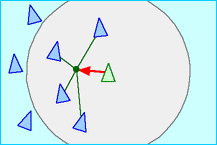
\includegraphics[width=0.3\textwidth]{flocking_cohesion}}
%  \subfloat[Repulsion]{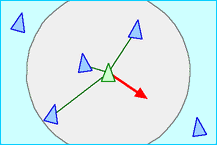
\includegraphics[width=0.3\textwidth]{flocking_separation}}
%  \subfloat[Alignment]{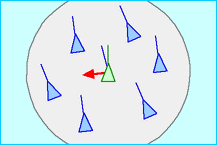
\includegraphics[width=0.3\textwidth]{flocking_alignment}}
%  \caption{Visual representation of the basic Boidean collision avoidance rules used}
%  \label{fig:boids}
%\end{figure*}


\subsection{Standards of Accuracy}\label{sec:standards}

The key question of this paper is to assess the advantages and disadvantages of utilising trust from the physical domain. 

It is important to clarify what is meant by ``effective'' in this case; the ``effectiveness'' of any trust assessment framework is taken as consisting of several parts, the \emph{accuracy} of detection and identification of a particular misbehaviour, the \emph{complexity} of such analysis, including any specific training required, and the \emph{differentiability} of behaviours using given metrics.

In this case we are particularly interested in the accuracy of detection and identification of malicious / failing behaviours, and as such are looking at three key characteristics of accuracy; true detection accuracy (what percentage of ``bad'' behaviours are detected at all); false positive rates (what percentage of ``control'' behaviours are detected as being ``bad''); and misidentification rates (how many instances of one bad behaviour are mischaracterised as the other and vie versa.

As such we have three primary questions to answer to establish if these metrics are useful: 
How accurate are these metrics in being able to easily differentiate between Normal and Abnormal behaviours in terms of True-Positive and False-Positive rates?
What differentiation of response, if any, is there between the stated abnormal behaviours?
Can a simple classification be built to characterise these differentiations of response, and what is it's True-Positive/False-Positive accuracy?


\subsection{Analysis}
Having established the metrics under investigation, 64 simulation runs are executed for each scenario (i.e.\ one node ``Maliciously'' following the fleet with no mission information (Shadow), one ``Failing'' node with simulated drive train issues (Shadow), and one baseline control scenario where all nodes are behaving appropriately (Control).
Each of these simulated missions last for an hour, matching realistic deployment times based on current MOD/NATO operations\cite{Bolster2014a}.

\subsubsection{Metric Cleaning}
In order to assess the viability of using the previously discussed metrics, the raw motion paths recorded by the simulation are fed into an analysis pipeline aimed at abstracting the instantaneous observed values into derived deviations from ``normal'' behaviour in the team.

\begin{align}
  d_{i,j}^{m,t} &= x_{i,j}^{m,t} - \frac{\sum_k x_{i,k}^{m,t}}{|M|}\label{eq:d}\\
  \alpha_{i,j}^{m,t} &= | \frac{d_{i,j}^{m,t}}{\sigma{d_{i,j}^{m,t}}}|\label{eq:dd}
\end{align}

Where $i$ and $j$ are indices denoting the current observer node and the current observed node respectively; $x$ is a summation index representing other nodes in the observers region of concern; $X$ is the vector of metrics from~\ref{eq:phys_vector}; $d$ is an intermediate value of the distance of a given observation from the mean, and $\alpha$ is a resulting normalised response value in terms of it's deviation from the mean.

\subsubsection{Behaviour Detection and Classification}
A simple misbehaviour detection is to apply Dixon's Q-test \cite{Dean1951} to the resultant $\sum\alpha$ values for each node for each metric for each run  a) establish if a ``misbehaving node'' exists in a given run, and b) identify that misbehaving node. 
For our initial investigation we will use a Confidence Interval of $95\%$.

Our initial hypothesis is that by using observations of the previously stated physical metrics, that we will be able to detect and identify misbehaviours.
Within that context, this Confidence Interval indicates that we would expect only a $5\%$ chance that any run or node identified using the Q-test to \emph{not} be a misbehaving run/node.
Further, due to the range of metrics available, by applying the Q-test on a per-metric basis, we can use the ``votes'' of each metric as a simplified consensus classifier.
This classifier may allow us to characterise some aspect of a given misbehaviour in terms of metrics it heavily impacts, and those that are less affected, finding some differentiating-limit between certain behaviours using certain metrics.

\begin{equation}
  C_{i}^{m} = \Sigma_t\sigma_{i}^m * \frac{N-1}{\sum_{x\neq i}{\Sigma_t\sigma_{x}^m}}\label{eq:confidence}
\end{equation}

\subsubsection{Operational Performance Metrics}
While not the focus of this paper, we are also concerned with the impact of these misbehaviours on the mission efficiency of the team overall.
We monitor this in three main measurements; the ``speed'' of the fleet in terms of how many of it's port-protection waypoints it successfully approaches and passes, the total energy used for communications, and the average end-to-end delay in the acoustic network.
We would expect that any misbehaviour in positioning will incur some loss of efficiency, whether it is the fleet being slowed down by a straggler attempting to catch up or of a node moving in an unexpected fashion dragging the team temporarily off course.
Given that in acoustic communications, transmission is energetically expensive while reception is not, and while physical misbehaviours will not impact the amount of offered load on the network, collisions induced by un-even distribution of nodes should have a small but measurable effect on energy used for packet reception.

\section{Results and Discussion}
Fig.~\ref{fig:metric_values} shows the raw metric values (vertically) from one run of each behaviour (horizontally), starting with the Control case, where all node are behaving properly.
The misbehaving node in the remaining cases.
It clear that using the (unitless) INDD and INHD metrics, Alfa is the outlier and other, fairly behaving, nodes are all consistent in their metric values.
This outlier-response is not nearly as clear in the Speed metric case (bottom row of Fig.~\ref{fig:metric_values}).

From a behaviour-perspective, it appears that the Shadow behaviour is creating the largest, most obvious deviations.

\begin{figure*}
  \centering
  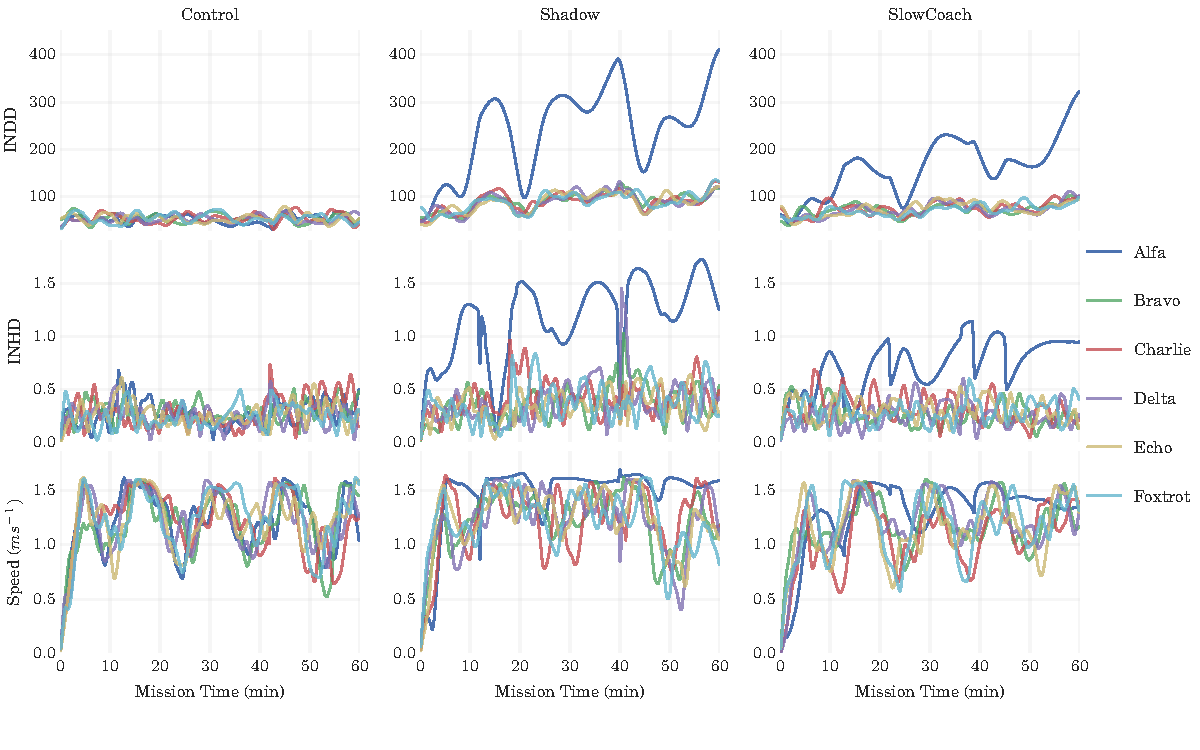
\includegraphics[width=0.8\textwidth]{Metric_Values}
  \caption{Observed Metric Values for one simulation of each behaviour ($x_{i,j}^{m,t}$ from \eqref{eq:d})}
  \label{fig:metric_values}
\end{figure*}

%\begin{figure*}
%  \centering
%  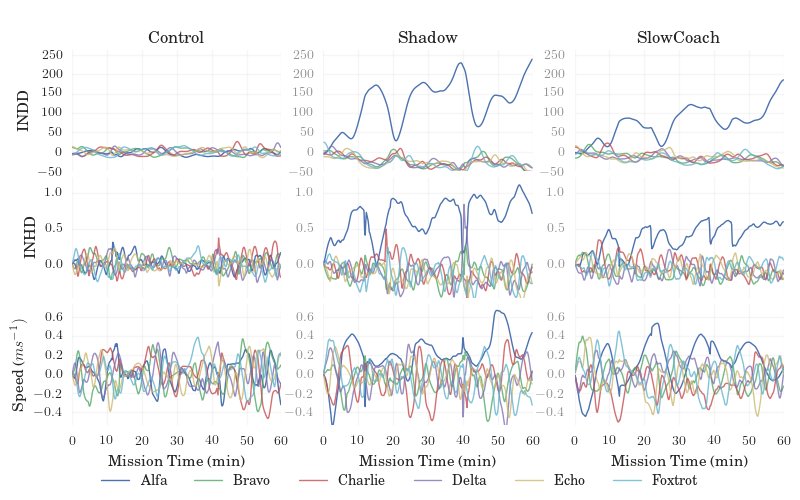
\includegraphics[width=0.8\textwidth]{Metric_Deviation}
%  \caption{\emph{Unnecessary but included for draft discussion} Observed Metric Values for one simulation of each behaviour ($d_{i,j}^{m,t}$ from Fig.~\ref{fig:workflow})}
%\end{figure*}

In Fig.~\ref{fig:deviance_values} the metric values are normalised as per \eqref{eq:dd}.
This has highlighted the outlying-characteristic of INHD and INDD; largely eliminating the other nodes-responses.
In the Speed response of Fig.~\ref{fig:deviance_values}, the Speed metric is not obviously highlighting any significant misbehaviours in that metric. 

\begin{figure*}
  \centering
  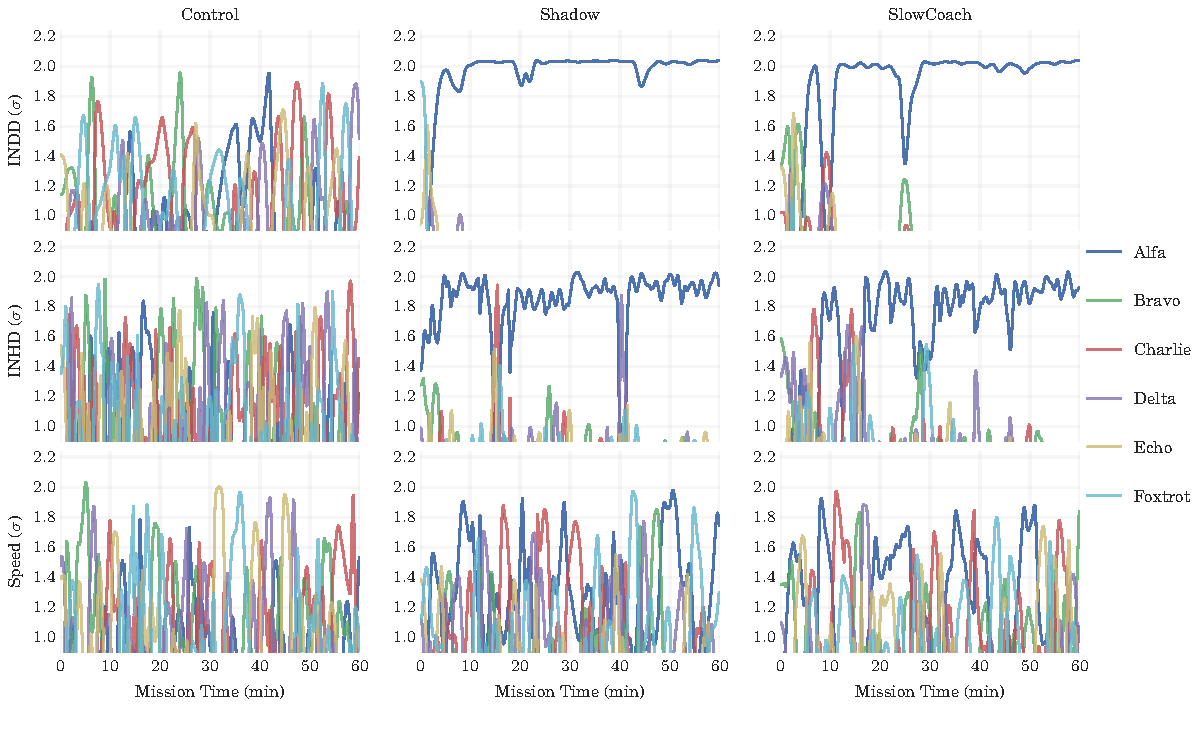
\includegraphics[width=0.8\textwidth]{Metric_Sigma_Deviance}
  \caption{Normalised Deviance values from one simulation of each behaviour ($\alpha_{i,j}^{m,t}$ from \eqref{eq:dd})}
  \label{fig:deviance_values}
\end{figure*}

From Fig.~\ref{fig:summedsigmabar}, it appears that Speed is being significantly affected by the differing behaviours, but much less so than INHD/INDD.  

\begin{figure*}
  \centering
  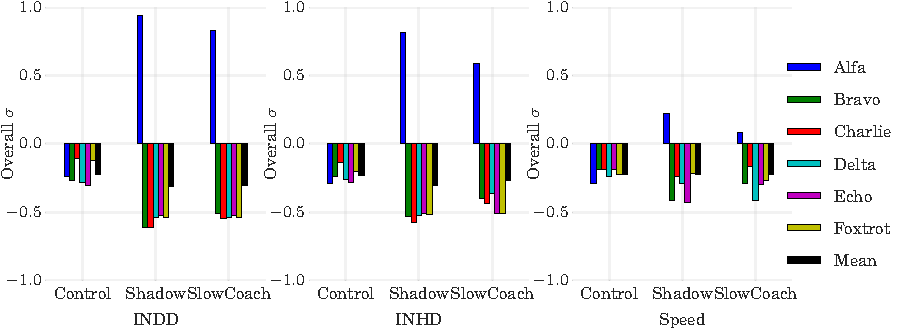
\includegraphics[width=\linewidth]{summedsigmabar}
  \caption{Per-Node-Per-Run deviance for each metric, normalised in time ($\sum\alpha/T$)}
  \label{fig:summedsigmabar}
\end{figure*}

\subsection{Detection of Misbehaviours}
We have demonstrated by graphical result that from our initial metrics, INHD and INDD do appear to accurately and obviously identify the malicious node in the case that there is one. 
Using the deviance normalisation presented in \eqref{eq:dd}, we can observe clear, almost contiguous areas under the Alfa-values in Fig.~\ref{fig:deviance_values} in the Shadow and SlowCoach misbehaviours.
Further, from Fig.~\ref{fig:summedsigmabar}, we have shown that while it is nowhere near as ``clear'' as the deviance in INHD and INDD, that the Speed metric is still registering a statistically significant deviation in both misbehaviours, and that the difference between the deviances in Speed may indicate a way to analytically differentiate between the two misbehaviours.

To investigate how this would relate to the ability to blindly detect misbehaviours, the Q-test is applied to $\Sigma\alpha$ results as used in Fig.~\ref{fig:summedsigmabar}, to attempt to correctly establish a) if a node is misbehaving and b) which node is misbehaving. 
As such the ``correctness'' rule for assessing this strategy is that, in misbehaving cases, the Q-tests should return Alfa (otherwise a ``Fail'' is recorded), and in the Control case, the Q-test should assert that there are no obvious outliers, (otherwise a ``Fail'' is recorded again).
In Table~\ref{tab:overall_stats}, the Null case (Control behaviour) is correctly identified 92\% of the time.
The ``malicious'', Shadow misbehaviour is detected and identified 98\% of the time, and the ``failing'', SlowCoach misbehaviour is identified just 79\% of the time. 
These values match our intuition from Figs.~\ref{fig:metric_values} and~\ref{fig:deviance_values}.

\begin{table}
  \caption{Overall Q-Test Outlier Correct Detection Accuracy}
  \centering
\begin{tabular}{lll}
\toprule
Behaviour &  Mean &   Std \\
\midrule
Control   & 0.927 & 0.261 \\
Shadow    & 0.979 & 0.144 \\
SlowCoach & 0.792 & 0.408 \\
\bottomrule
\end{tabular}
  %\begin{tabular}{lll}
\toprule
{} &  Mean &   Std \\
Behaviour &       &       \\
\midrule
Control   & 0.927 & 0.261 \\
Shadow    & 0.979 & 0.144 \\
SlowCoach & 0.792 & 0.408 \\
\bottomrule
\end{tabular}

  \label{tab:overall_stats}
\end{table}

We can investigate this further by looking at the ``correctness'' of the assessments of each metric individually (Table~\ref{tab:per_metric_stats}).
From this we can see that in both misbehaviours, INHD and INDD correctly identify Alfa as the misbehaver 100\% of the time. 
However, they misidentify a potential misbehaviour in the Control case 13\% and 7\% of the time respectively.
Meanwhile, Speed correctly identified the Control case 97\% of the time, and the Shadow case 94\% of the time, but missed the SlowCoach behaviour 63\% of the time. 
This result is surprising on the face of it, as SlowCoach is a misbehaviour that is exclusively about individual node speed and conceptually should have had a much larger impact on the simple Speed metric.
However, the collaborative nature of the collision avoidance system, and the existing limits on node kinematics from Table~\ref{tab:mobility_sysconstraints} appear to be hiding this impact. 

\begin{table}
  \caption{Per-Metric Q-Test Outlier Detection Accuracy}
  \centering
\begin{tabular}{lllll}
\toprule
{} & Behaviour &  INDD &  INHD & Speed \\
\midrule
Mean & Control & 0.875 & 0.938 & 0.969 \\
     & Shadow & 1.000 & 1.000 & 0.938 \\
     & SlowCoach & 1.000 & 1.000 & 0.375 \\
Std & Control & 0.336 & 0.246 & 0.177 \\
     & Shadow & 0.000 & 0.000 & 0.246 \\
     & SlowCoach & 0.000 & 0.000 & 0.492 \\
\bottomrule
\end{tabular}
  %\begin{tabular}{lllll}
\toprule
     &         &  INDD &  INHD & Speed \\
{} & Behaviour &       &       &       \\
\midrule
mean & Control & 0.875 & 0.938 & 0.969 \\
     & Shadow & 1.000 & 1.000 & 0.938 \\
     & SlowCoach & 1.000 & 1.000 & 0.375 \\
std & Control & 0.336 & 0.246 & 0.177 \\
     & Shadow & 0.000 & 0.000 & 0.246 \\
     & SlowCoach & 0.000 & 0.000 & 0.492 \\
\bottomrule
\end{tabular}

  \label{tab:per_metric_stats}
\end{table}

\subsection{Identification of Misbehaviours}
Having established the ability of INDD, INHD and Speed to all detect physical misbehaviour to a statistically significant level, and that there is a demonstrable difference in response to different misbehaviours,  we now focus on our last question from Sec.~\ref{sec:standards}; can we construct a simple classifier based on a subset of our results and apply it blindly to a new set of results?

From~\eqref{eq:confidence}, we can establish the per-metric-per-behaviour ``Confidence'' in the relationship between a given metric deviance and each behaviour. We hypothesise that this confidence can be used as a signature for that metric.

%\begin{table}[h]
%  \caption{Metric Confidence Responses for known behaviours~\eqref{eq:confidence}}
%  \centering
%\begin{tabular}{lrrr}
%\toprule
%metric &  INDD &  INHD &  Speed \\
%var       &       &       &        \\
%\midrule
%Control   & 0.970 & 0.914 &  0.892 \\
%Shadow    & 4.459 & 3.875 &  1.797 \\
%SlowCoach & 3.910 & 2.847 &  1.518 \\
%\bottomrule
%\end{tabular}
%\end{table}
\begin{table}[h]
  \caption{Metric Confidence Responses for known behaviours~\eqref{eq:confidence}}
  \centering
\begin{tabular}{llrrr}
\toprule
{} & Behaviour &  INDD &  INHD &  Speed \\
\midrule
Mean & Control & 1.064 & 0.966 &  1.010 \\
     & Shadow & 4.059 & 3.374 &  2.098 \\
     & SlowCoach & 4.246 & 3.352 &  1.491 \\
Std & Control & 0.262 & 0.113 &  0.132 \\
     & Shadow & 0.398 & 0.436 &  0.206 \\
     & SlowCoach & 0.198 & 0.288 &  0.180 \\
\bottomrule
\end{tabular}
  %\begin{tabular}{lrrr}
\toprule
metric &  INDD &  INHD &  Speed \\
var       &       &       &        \\
\midrule
Control   & 0.970 & 0.914 &  0.892 \\
Shadow    & 4.459 & 3.875 &  1.797 \\
SlowCoach & 3.910 & 2.847 &  1.518 \\
Tail      & 4.183 & 3.658 &  2.116 \\
\bottomrule
\end{tabular}

  \label{tab:confidence}
\end{table}

As we can already establish the Null case to a strong degree of accuracy, our classifier will continue to use the Q-test across all metrics for that case and concentrate of differentiating the Shadow and SlowCoach behaviours. 

From Table~\ref{tab:confidence} we observe that INHD and INDD have similar responses to both misbehaviours, with significant standard deviations, but the response of the Speed metric is much more stable and discernible; across the range of training simulation runs, the SlowCoach behaviour centres around $1.5$, while the Shadow behaviour centres around $2.0$, with these centres being at least one standard deviation away from each other.
Our generated classifier is formalised in~\eqref{eq:classifier}.

\begin{equation}
  C \rightarrow 
  \begin{cases}
    % Control
    Q^{95}(X) = \emptyset,& \text{Control}\\
    % Shadow
    Q^{95}(X) \neq \emptyset \land \text{Speed}^X \leq 1.75, & \text{Shadow}\\
    % SlowCoach
    Q^{95}(X) \neq \emptyset \land \text{Speed}^X > 1.75,& \text{SlowCoach}\\
  \end{cases}
  \label{eq:classifier}
\end{equation}

Applying this simplified classifier to a blind test set of simulations (of the same scale) gives surprisingly positive results as shown in Table~\ref{tab:classifier}, with greater than 90\% identification rates for both misbehaviours.
However, in this case we experience a false-positive rate of nearly 30\%.
Given the simplicity of the applied classifier, this is a strongly positive result for the use of physical metrics for behaviour discrimination; with INHD and INDD proving as strong and obvious ``canaries'' of misbehaviour, and Speed in this case proving a capable differentiator between conceptually close misbehaviours.

\begin{table}[h]
  \caption{Successful Identification rates on untrained results using~\eqref{eq:classifier}}
  \centering
  \begin{tabular}{lr}
    \toprule
    True Behaviour &  Probability of Correct Blind Identification \\
    \midrule
    Control        &                                        0.719 \\
    Shadow         &                                        0.906 \\
    SlowCoach      &                                        0.938 \\
    \bottomrule
  \end{tabular}
  %\begin{tabular}{lr}
\toprule
{} &  Probability of Correct Blind Identification \\
True Behaviour &                                              \\
\midrule
Control        &                                        0.719 \\
Shadow         &                                        0.906 \\
SlowCoach      &                                        0.938 \\
\bottomrule
\end{tabular}

  \label{tab:classifier}
\end{table}

%\begin{table}[h]
%  \caption{Successful Identification rates on untrained results using~\eqref{eq:classifier}, with outlier concensus checks}
%  \centering
%  \begin{tabular}{lr}
\toprule
{} &  Probability of Correct Blind Identification \\
True Behaviour &                                              \\
\midrule
Control        &                                        1.000 \\
Shadow         &                                        0.906 \\
SlowCoach      &                                        0.938 \\
\bottomrule
\end{tabular}

%  \label{tab:classifier_minority}
%\end{table}



\subsection{Impacts of Misbehaviour on operational performance}
The anticipated ``small but measurable'' effects to communications performance and energy usage are indeed extremely small and within the bounds of statistical uncertainty.
One observation of merit was an observed 10\% increase in end-to-end delay in the case of the Shadow behaviour; this is due to the misbehaving node ``overshooting'' the mission waypoints and thus temporarily looking local connection to nodes on the opposite side of the fleet from it, causing retransmissions thus, delays.
As for physical efficiency, achievement rates were identical to within 2\% error on each run across all behaviours, and fleet distance varied by a similar margin.
It's possible that our selected behaviours were too unambitious in our impacts, and future work will have to investigate the impact of ``heavy-handed'' or destructive behaviours on the operational efficiency of autonomous networks.

\section{Conclusion}
In this paper we have demonstrated that with current and on-the-horizon underwater localisation techniques, that in certain mobility models, that a set of relatively simple geometric abstractions (INHD, INDD, and Speed), between nodes as part of an Underwater MANET can be used as a Trust Assessment and Establishment metric.

These metrics are application-agnostic and could potentially be applied in other areas of mobile autonomy such as UAV operations and Autonomous Vehicular Networks.

We show, using a Port-Protection waypoint-led scenario built upon a Boidian collision prevention behaviour that in a simulated underwater environment, the outputs of these metrics can be used to detect and differentiate between exemplar malicious behaviour and potential failure states.

This verification further supports the assertions the authors have made previously that it is practical to extend Trust protocols such as Multi-parameter Trust Framework for MANETS (MTFM)\cite{Guo2012} to include metrics and observations from the physical domain as well as those from the communication domain\cite{Bolster2014}.
This combination of physical and ``logical'' information would further support the decentralised and distributed establishment of observation based Trust.


% conference papers do not normally have an appendix


% use section* for acknowledgement
\section*{Acknowledgment}

The Authors would like to thank the DSTL/DGA UK/FR PhD Programme for their support during this project, as well as NATO CMRE for their advice and assistance.

\bibliographystyle{IEEEtran}
% argument is your BibTeX string definitions and bibliography database(s)
\bibliography{IEEEabrv,refs}

% that's all folks
\end{document}


% An example of a floating figure using the graphicx package.
% Note that \label must occur AFTER (or within) \caption.
% For figures, \caption should occur after the \includegraphics.
% Note that IEEEtran v1.7 and later has special internal code that
% is designed to preserve the operation of \label within \caption
% even when the captionsoff option is in effect. However, because
% of issues like this, it may be the safest practice to put all your
% \label just after \caption rather than within \caption{}.
%
% Reminder: the "draftcls" or "draftclsnofoot", not "draft", class
% option should be used if it is desired that the figures are to be
% displayed while in draft mode.
%
%\begin{figure}[!t]
%\centering
%\includegraphics[width=2.5in]{myfigure}
% where an .eps filename suffix will be assumed under latex, 
% and a .pdf suffix will be assumed for pdflatex; or what has been declared
% via \DeclareGraphicsExtensions.
%\caption{Simulation Results}
%\label{fig_sim}
%\end{figure}

% Note that IEEE typically puts floats only at the top, even when this
% results in a large percentage of a column being occupied by floats.


% An example of a double column floating figure using two subfigures.
% (The subfig.sty package must be loaded for this to work.)
% The subfigure \label commands are set within each subfloat command, the
% \label for the overall figure must come after \caption.
% \hfil must be used as a separator to get equal spacing.
% The subfigure.sty package works much the same way, except \subfigure is
% used instead of \subfloat.
%
%\begin{figure*}[!t]
%\centerline{\subfloat[Case I]\includegraphics[width=2.5in]{subfigcase1}%
%\label{fig_first_case}}
%\hfil
%\subfloat[Case II]{\includegraphics[width=2.5in]{subfigcase2}%
%\label{fig_second_case}}}
%\caption{Simulation results}
%\label{fig_sim}
%\end{figure*}
%
% Note that often IEEE papers with subfigures do not employ subfigure
% captions (using the optional argument to \subfloat), but instead will
% reference/describe all of them (a), (b), etc., within the main caption.


% An example of a floating table. Note that, for IEEE style tables, the 
% \caption command should come BEFORE the table. Table text will default to
% \footnotesize as IEEE normally uses this smaller font for tables.
% The \label must come after \caption as always.
%
%\begin{table}[!t]
%% increase table row spacing, adjust to taste
%\renewcommand{\arraystretch}{1.3}
% if using array.sty, it might be a good idea to tweak the value of
% \extrarowheight as needed to properly center the text within the cells
%\caption{An Example of a Table}
%\label{table_example}
%\centering
%% Some packages, such as MDW tools, offer better commands for making tables
%% than the plain LaTeX2e tabular which is used here.
%\begin{tabular}{|c||c|}
%\hline
%One & Two\\
%\hline
%Three & Four\\
%\hline
%\end{tabular}
%\end{table}


% Note that IEEE does not put floats in the very first column - or typically
% anywhere on the first page for that matter. Also, in-text middle ("here")
% positioning is not used. Most IEEE journals/conferences use top floats
% exclusively. Note that, LaTeX2e, unlike IEEE journals/conferences, places
% footnotes above bottom floats. This can be corrected via the \fnbelowfloat
% command of the stfloats package.


